\documentclass[main.tex]{subfiles}
\begin{document}
\begin{enumerate}

\item[1.] \textbf{Decision Trees (10pt):} In class we discussed the example of buying a car and the bank using a Decision Tree to decide whether a client is in the high or low risk category for the loan. Our tree had 2 decision steps. \textbf{Q:} Redo the tree, but design it with a only a single decision step. Show that tree. 

\begin{algorithm}
\caption{A singe step decision tree}
\begin{algorithmic}[1]
\If{$income > x$}
    \State approve loan
\Else
    \State reject loan
\end{algorithmic}
\end{algorithm}

\textbf{Q:} What role has the no in this case? \textbf{A:} Low savings low income, and high savings low income.

\item[2.] \textbf{Perceptron - Warm-up (5pts each = 40pt):} \textbf{Q:} We call the model ‘neuromorphic’ (bio-inspired). Show the functions of biological cell versus the Perceptron model. \textbf{A:} A real neurons structure includes Dendrites $\rightarrow$ Axon (Myelin sheath) $\rightarrow$ Axon terminals. Artificial neurons have axons from a neuron $x_i$ and synapses $w_i$ connect via dendrites to cell body $\sum_{i} w_i x_i +b$. \textbf{Q:} What are the inputs called? \textbf{A:} Inputs and weights. \textbf{Q:} State the parameters of the perceptron algorithm including their name, symbol, and whether it’s a scalar, vector, or matrix? \textbf{A:} Input vector $\vec{x}$, weights vector $\vec{w}$, and bias scalar $b$. \textbf{Q:} What mathematical function is the response? \textbf{A:} The response in the form of the activation function producing a real number $a=\sum_{d=1}^{D} w_d x_d + b$. \textbf{Q:} What is the output if the response is positive or negative? \textbf{A:} If the activation value is negative the label $y$ is set to -1, and if the activation value is positive the label $y$ is set to +1. \textbf{Q:} At what point does an error occur between the mathematical relationship between $y$ and $a$? \textbf{A:} During training we only update weights and biases when $ya \leq 0$ because when $y = -1$  the current prediction is incorrect. \textbf{Q:} When an error is made during training what does the updated weight $w^{\prime}$ equal? \textbf{A:} $w^{\prime} = w - x$ because $w_d^{\prime} = w_d + yx$ and during an error $y=-1$. \textbf{Q:} What is the activation value exactly at the decision-boundary $B$? What is $a$ above and below $B$? \textbf{A:} At the decision boundary $B$ the value of the activation function $a$ changes from negative to positive and is zero along the boundary.    

\item[3.] \textbf{Perceptron Model (20pt):} We discussed the perceptron training algorithm (e.g. Algorithms #5, from Daume, p. 43) in class. \textbf{Q:} Is it important to check whether the product or label and activation function are smaller than or equal to zero, or could we simply check for smaller than zero? Write an explanation of why you think the ‘equal’ symbol is, or is not relevant during perceptron training. \textbf{A:} $ya \leq 0$ is correct, and $ya < 0$ is incorrect when it comes to deciding if weights and bias should be updated during perceptron training. When $ya=0$ we know that the activation value  $a=0$ because the label $y$ can only equal +1 or -1. If the activation $a$ is positive it predicts that the current example is a positive example. Otherwise it predicts a negative example. Therefore 0 is a negative case. 

\item[4.] \textbf{Perceptron Training Algorithm (3x10 = 30pt):} \textbf{Q Part-1:} We discussed the perceptron training Algorithm in class for an exemplary 'positive' example (i.e. y = +1). We found that the training algorithm (correctly so) increases the activation. Does this algorithm also work if the sample is 'negative'? Work out the training steps for a 'negative' example. Does it still work? Why?  \textbf{A:}
$\vec{w} = \begin{bmatrix} -1 \\ 1 \\ -3 \\ \end{bmatrix}$ $\vec{x} = \begin{bmatrix} 2 \\ 3 \\ 1 \\ \end{bmatrix}$ $b=0$ $\sum_i w_i x_i +b = -2$ $\therefore y = -1$ The algorithm works if the activation value is negative because it sets the label to -1 which indicates an incorrect prediction and during training initiates a recalculation of weights and biases. \textbf{Q Part-2:} We discussed the geometrical interpretation of the perceptron’s ‘job’, i.e. to create a decision boundary $B$, that successfully and geometrically (i.e. spatially) separates the data, i.e. a plane of scattered data points in a 3-dimensional space. Graphically sketch the dot-product between the 2 vectors, such as between the weights and inputs (\textbf{A:} Figure \ref{fig:1}).  Here (Figure \ref{fig:2}), we have data in a 2D plane (x1, and x2). 
\begin{figure}
\centering\fbox{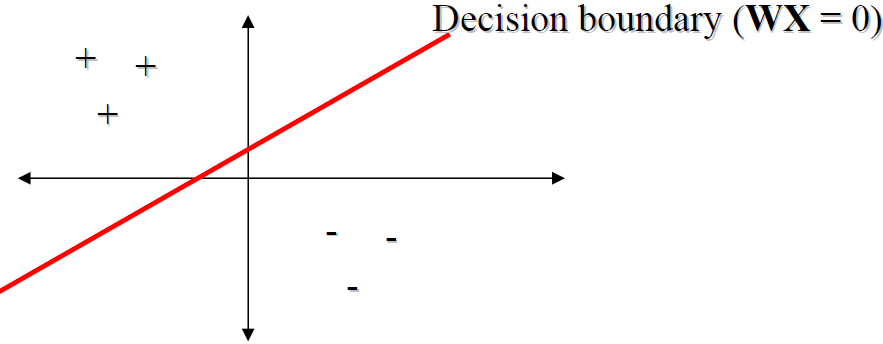
\includegraphics[height=2.0in]{figures/hw2/hw2_1.png}}
\caption{Decision boundary}
\label{fig:1}
\end{figure}
\begin{figure}
\centering\fbox{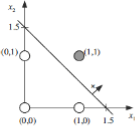
\includegraphics[height=2.0in]{figures/hw2/hw2_2.png}}
\caption{2D plane}
\label{fig:2}
\end{figure}
The boundary (here a line), separates data. What does the output function look like for this? What it the bias $b$, and hence, what mathematical function does this data-set represent? \textbf{A:} $x_2 = x_1 + 1.5$, $b = 1.5$, $a =\sum_i w_i x_{i} + 1.5$. The data points form a square and the the decision boundary function is linear. \textbf{Q Part-3:} If permuting the data each iteration saves somewhere between 20\% and 50\% of your time, are  there any cases in which you might not want to permute the data every iteration? State your answer, and give an explanation. Provide 2 data set examples: one where permutations help and some where it will (likely) not help. \textbf{A:} Changing the data sets permutation between each training iteration is helpful when the variance in the data set is relatively high. The higher the variance the more helpful permeation will be during training.

\end{enumerate}
\end{document}